%% packages
\documentclass{article}
\usepackage[a4paper, left=2.0cm, right=2.0cm, top=3.5cm]{geometry}
\usepackage[ngerman]{babel}
\usepackage{graphicx}
\usepackage{multicol}
\usepackage{amssymb}
\usepackage{titlesec}
\usepackage{wrapfig}
\usepackage{blindtext}
\usepackage{lipsum}
\usepackage{caption}
\usepackage{listings}
\usepackage{fancyhdr}
\usepackage{nopageno}
\usepackage{authblk}
\usepackage{amsmath} % tons of math stuff
\usepackage{mathtools} % e.g. alignment within matrix
%\usepackage{bm} % provides shorthand for bold in math mode
\usepackage{dsfont} % \mathds makes double stroke digits
\usepackage{esdiff} % provides \diff
%\usepackage[ISO]{diffcoeff}
\usepackage{xcolor}
\usepackage{csquotes} % e.g. provides \enquote
\usepackage[separate-uncertainty=true]{siunitx} % units
\usepackage{xcolor} % colored text
\usepackage{csvsimple}
\usepackage{subcaption}
\usepackage{physics}
\usepackage{hyperref}
\usepackage{nameref}
\hypersetup{colorlinks=true, linkcolor=black, pdfhighlight={/N}}
\usepackage{tcolorbox}
\usepackage{amsthm}




%\fancyhf[]{}

%% custom stuff
% own units
\DeclareSIUnit \VSS {\ensuremath{V_\mathrm{SS}}}
\DeclareSIUnit \VS {\ensuremath{V_\mathrm{S}}}
\DeclareSIUnit \Veff {\ensuremath{V_\mathrm{eff}}}
\DeclareSIUnit \Vpp {\ensuremath{V_\mathrm{pp}}}
\DeclareSIUnit \Vp {\ensuremath{V_\mathrm{p}}}
\DeclareSIUnit \VRMS {\ensuremath{V_\mathrm{RMS}}}
\DeclareSIUnit \ASS {\ensuremath{A_\mathrm{SS}}}
\DeclareSIUnit \AS {\ensuremath{A_\mathrm{S}}}
\DeclareSIUnit \Aeff {\ensuremath{A_\mathrm{eff}}}
\DeclareSIUnit \App {\ensuremath{A_\mathrm{pp}}}
\DeclareSIUnit \Ap {\ensuremath{A_\mathrm{p}}}
\DeclareSIUnit \ARMS {\ensuremath{A_\mathrm{RMS}}}

% change subsection numbering to capital letters
\newcommand{\subsectionAlph}{ \renewcommand{\thesubsection}{\arabic{section}.\Alph{subsection}} }
% change subsection numbering to lowercase letters
\newcommand{\subsectionalph}{ \renewcommand{\thesubsection}{\arabic{section}.\alph{subsection}} }
% change subsubsection numbering to lowercase letters
\newcommand{\subsubsectionalph}{ \renewcommand{\thesubsubsection}{\arabic{section}.\arabic{subsection}.\alph{subsubsection}} }
% own fig. that works with multicols
\newenvironment{Figure}
  {\par\medskip\noindent\minipage{\linewidth}}
  {\endminipage\par\medskip}
\newcommand*{\inputPath}{./plot} % prepend this command to the argument of all input commands
\graphicspath{ {./images/}{./figure/}{../plot/} }
% own enviroment for definitions
\newenvironment{definition}[1]
{\begin{quote} \noindent \textbf{\textit{#1\ifx&#1& \else : \fi}} \itshape}
{\end{quote}}


% own commands
% \newcommand{\rarr}{$\to\,$} %A$\,\to\,$B
\newcommand{\defc}{black}
\newcommand{\colorT}[2][blue]{\color{#1}{#2}\color{\defc}}
\newcommand{\redq}{\color{red}(?)\color{\defc}}
\newcommand{\question}[1]{\colorT[purple]{\textbf{(#1)}}}
\newcommand{\todo}[1]{\colorT[red]{\textbf{(#1)}}}
\newcommand{\mr}{\mathrm}

%% preparation
\begin{titlepage}
    \title{Praktikum Atome, Moleküle, kondensierte Materie \\ Versuch 401}
    \author[1]{Carlos Pascua\thanks{s87cpasc@uni-bonn.de}}
    \author[1]{Michael Vogt\thanks{s65mvogt@uni-bonn.de}}
    \affil[1]{Uni Bonn}
    %\date{\today}
\end{titlepage}


%% document
\begin{document}

\pagenumbering{gobble}
\maketitle
\tableofcontents
\newpage
\pagenumbering{arabic}

\pagestyle{fancy}
\fancyhead[R]{\thepage}
\fancyhead[L]{\leftmark}

\begin{multicols}{2}

\section*{Einleitung}


\section{Durchführung \& Auswertung}

\clearpage
\section{Teil ll: Franck-Hertz-Versuch}
Im folgenden Abschnitt wird das Franck-Hertz-Experiment durchgeführt und anschließend detailliert 
diskutiert. Anhand der durch das Cassy-Modul gemessenen Anodenstromkurven \( I_A \) wird die 
Energiedifferenz \( \Delta E \) zwischen den Energieniveaus des Quecksilbers, \( 6S \) und \( 6P \), 
präzise bestimmt.

\subsection{Aufbau}
In einer Franck-Hertz-Röhre, die mit Quecksilbers gefüllt ist, befindet sich eine glühende 
Kathode mit einer Heisspannung $U_H$, die die Elektronen durch thermische Emmission freisetzt und in der 
Richtung einer positiv geladenen Anode beschleunigt. Die Beschleunigungsspannung $U_B$ zwischen Kathode 
und Anode bestimmt die kinetische Energie der Elektronen, bevor sie auf die Quecksilberatome treffen.

Zwischen der Kathode und der Anode befindet sich ein Gitter, das in einigen Konstruktionen mit einem kleinen 
Gegenfeld ausgestattet ist, um Elektronen, die nach elastische nd inelastische Stößen ihre kinetische Energie 
verloren haben, daran zu hindern, die Anode zu erreichen. Der Anodenstrom $I_A$
wird dann in Abhängigkeit von der Spannung $U_B$ gemessen. Bei bestimmten Spannungswerten zeigt der Anodenstrom charakteristische Einbrüche, die auftreten, wenn die Elektronen genau die Energie erreichen, die nötig ist, um ein Quecksilberatom vom Grundzustand (6S) in einen angeregten Zustand (6P) zu heben.
 Durch diesen inelastischen Stoß verlieren die Elektronen ihre kinetische Energie und tragen dadurch nicht mehr zum Stromfluss bei.

Die Spannungsdifferenz zwischen aufeinanderfolgenden Strommaxima liefert die Energie $\Delta E$, die den 
Übergang zwischen den 6S- und 6P-Niveaus beschreibt. 

\subsection{Durchführung und Auswertung}
\begin{figure}[h!]
  \centering
  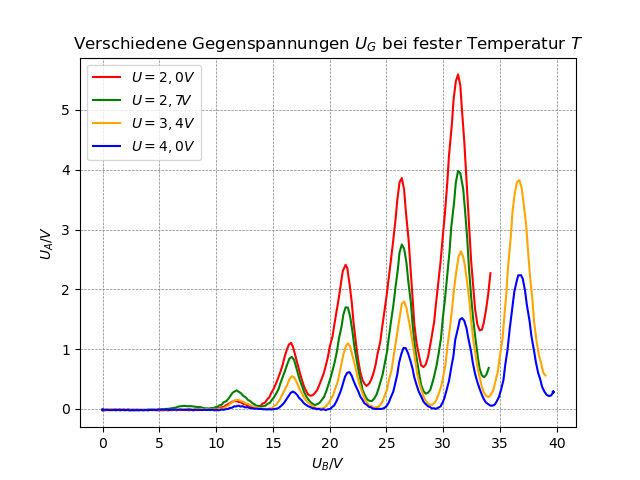
\includegraphics[scale=0.4125]{../p401/latex/figure/FH_vieleT.png}
  \caption{Bestimmung der Funktion für $N=2$}
\end{figure}


\begin{figure}[h!]
  \centering
  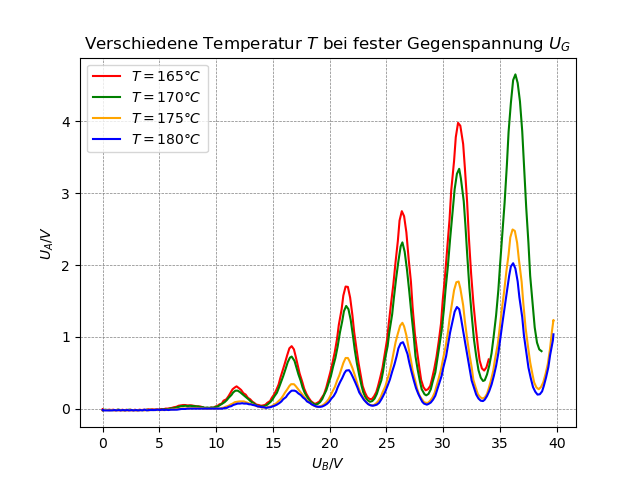
\includegraphics[scale=0.4125]{../p401/latex/figure/FH_vieleU.png}
  \caption{Bestimmung der Funktion für $N=2$}
\end{figure}

\clearpage
\section{Fazit}


\clearpage
\begin{thebibliography}{9}

\bibitem{Anleitung}
\textit{Physikalisches Praktikum Teil IV -- Versuchsbeschreibungen}, Universität Bonn, 10.10.2024


\end{thebibliography}

\end{multicols}

\end{document}

